\documentclass[12pt]{article}
\usepackage[utf8]{inputenc}
\usepackage[a4paper, top=2cm, bottom=2cm, left=2cm, right=2cm]{geometry}
\usepackage[T1]{fontenc}
\usepackage[brazil]{babel}
\usepackage{amsmath, amssymb, amsthm,dsfont}
\usepackage{enumitem}
\usepackage{booktabs}
\usepackage{caption}
\usepackage{graphicx} % needed for images
\usepackage{bm} % para vetor em negrito \bm{x}

% Comando para qui-quadrado
\newcommand{\chisq}{\chi^2}

\begin{document}

\section*{Atividade 3 -- Planejamento}
Aluno: Marcelo Huang\\

\textbf{Enunciado:}  
Encontre um conjunto de dados adequado para a aplicação de um modelo ANOVA um fator (one-way).
Realize uma análise completa, incluindo a descrição do problema, a descrição dos dados,
 a verificação dos pressupostos do modelo (caso já possua esse conhecimento), 
 a construção da tabela ANOVA, 
 a execução do teste ANOVA 
 e a interpretação dos resultados.

Apresente o relatório em formato PDF (no Classroom) 
e elabore uma apresentação em slides desse relatório 
(você poderá ser solicitado a apresentá-lo em sala de aula). 
40\% dos pontos da avaliação serão atribuídos ao relatório em PDF e 60\% à apresentação.

\subsection*{Descrição}

\textbf{ Dados escolhidos: "morley"}
\\

Em 1879, dois físicos Albert Michelson e Edward Morley queriam medir a velocidade da luz.
Eles fizeram 5 tipos diferentes de experimentos, em cada tipo de experimento fizeram 
20 observações, depois registraram os dados sobre velocidades medidas.

Note que os dados do R são subtraídos por 299000 para simplicidade,
 e a unidade de medida é km/segundo.

O interesse dessa atividade é investigar se em média os experimentos possuem diferenças 
na medição da velocidade da luz.

\subsection*{Métodos}

Nessa atividade são usadas ferramentas estatísticas como: testes da normalidade(para verificar suposições necessárias 
para aplicaçãodo modelo ANOVA um fator),
gráficos exploratórios(para visualizar o comportamento dos dados),
medidas descritivas, tabela ANOVA e entre outras.

\begin{table}[ht]
\centering
\begin{tabular}{c c c c c}
\hline
Exp 1 & Exp 2 & Exp 3 & Exp 4 & Exp 5\\
\hline
850 & 960 & 880 & 890 & 890\\
740 & 940 & 880 & 810 & 840\\
900 & 960 & 880 & 820 & 780\\
1070 & 880 & 810  & 800 & 810\\
\vdots & \vdots & \vdots & \vdots & \vdots \\
960 & 800 & 840  & 780 & 870\\
\hline
\end{tabular}
\caption{Velocidades da luz em km/s (-299000) medidas nos experiementos }
\end{table}

\subsection*{Solução:}

São $a = 5 $ níveis de tratamentos. Para cada nível são feitos $n = 20$ ensaios.

Então temos que a hipótese nula é que as médias das velocidades são iguais, 
logo a hipótese alternativa é que existe uma diferença as médias das velocidades entre tratamentos.

\[
H_0: \mu_1 = \mu_2 = \mu_3 = \mu_4 = \mu_5
\]

\[
H_1: \text{Existe uma diferença nas médias entre tratamentos.}
\]

Usando ferramentas, são encontrados estatísticas descritivas para cada tratamento.
See Table 2.

\begin{table}[ht]
\centering
\begin{tabular}{lccccc}
\toprule
Tratamento & N & Média & Desvio Padrão & Mínimo & Máximo \\
\midrule
Exp 1 & 20 & 909 & 104.93 & 650 & 1070 \\
Exp 2 & 20 & 856 & 61.16 & 760 & 960 \\
Exp 3 & 20 & 845 & 79.11 & 620 & 970 \\
Exp 4 & 20 & 820.5 & 60.04 & 720 & 920 \\
Exp 5 & 20 & 831.5 & 54.22 & 740 & 950 \\
\bottomrule
\end{tabular}
\caption{Estatísticas descritivas para cada tratamento}
\end{table}

\subsection*{Verificando suposições:}
É necessário verificar se as suposições de normalidade e homocedasticidades são satisfeitas.

\begin{figure}[htbp]
    \centering
    \begin{minipage}{0.45\textwidth}
        \centering
        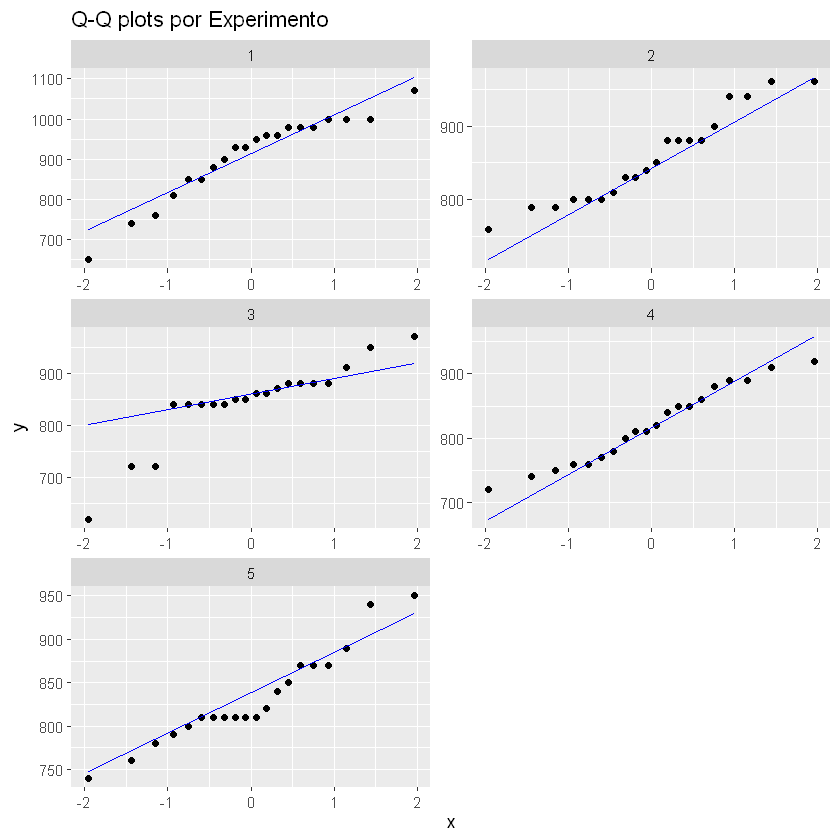
\includegraphics[width=\linewidth]{atv3 qqplot.png}
        \captionof{figure}{Q-Q plots para verificar a normalidade}
        \label{fig:qqplot}
    \end{minipage}
    \hfill
    \begin{minipage}{0.45\textwidth}
        \centering
        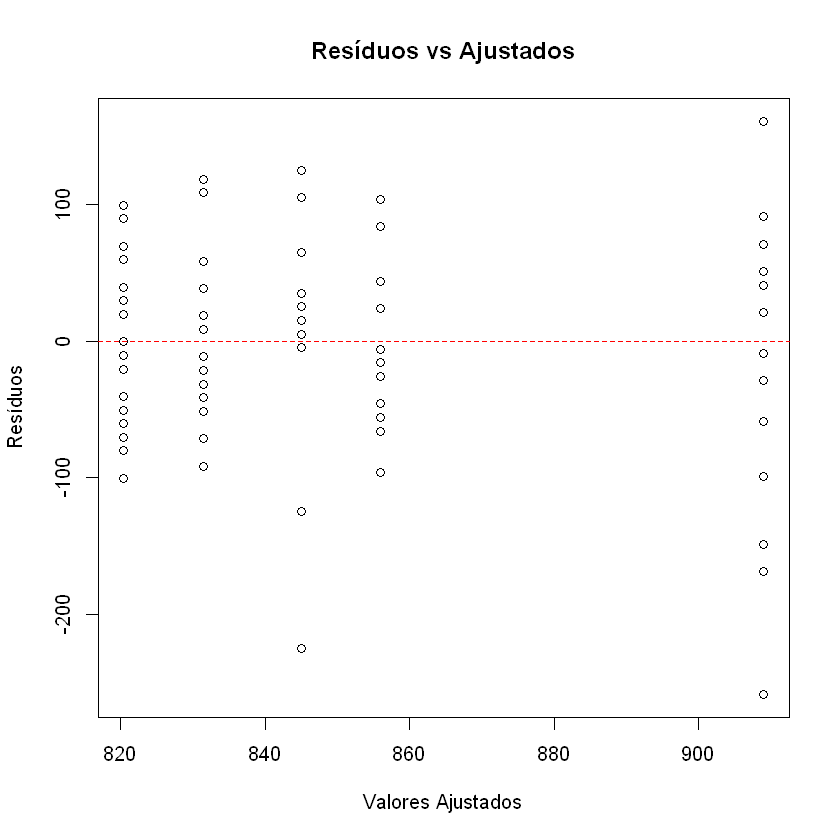
\includegraphics[width=\linewidth]{atv3 residuos vs ajustados.png}
        \captionof{figure}{Gráfico de resíduos para verificar a homocedasticidade}
        \label{fig:residuos}
    \end{minipage}
\end{figure}

Pelos Q-Q plots da figura 1, não há indícios visuais de alguma violação severa da suposição da normalidade,
já que a maioria dos pontos estão próximos de qq-line. Assim é aceita a suposição da normalidade.\\
Considerando os valores de desvios padrões da tabela 2 e o gráfico de residuos da figura 2, 
os desvios são, de um ponto de vista grossa, similares, e o espalhamento dos resíduos não são muito diferentes,
então é assumido que a suposição de variâncias iguais está satisfeita.
\\\\\\\\\\\\\\
\subsection*{Resultados: teste ANOVA}

\begin{table}[ht]
\centering
\begin{tabular}{lccccc}
\toprule
Origem & GL & SS & MS & Valor de F & Valor-p \\
\midrule
Tratamento & 4 & 94514 & 23629 & 4.288 & 0.00311 \\
Resíduos & 95 & 523510 & 5511 \\
\bottomrule
\end{tabular}
\caption{Análise de Variância}
\end{table}

A estatístiaca F de 4.288 é significativa e o valor-p $= 0.00311$ é próximo de zero,
então a hipótese nula é rejeitada.
Os dados ofereceram evidências suficientes para concluir que a média das velocidades medidas
dos diferentes experimentos são diferentes, ou seja, já que $H_0$ rejeitada, pelo menos uma média
de um tratamento é diferente das outras.
\end{document}